\documentclass[a4paper, 12pt, oneside, table]{article}
\usepackage[square, numbers, comma, sort&compress]{natbib}  % Use the "Natbib" style for the references in the Bibliography
\usepackage{verbatim} 
\usepackage[english]{babel}
\usepackage[utf8]{inputenc}
\usepackage{graphicx}
\usepackage{multirow}
\usepackage{amsmath}
\usepackage{amssymb}


%\usepackage{cite}
\usepackage{booktabs}
\usepackage{listings}
\usepackage{epstopdf}
\usepackage{helvet} 
\renewcommand{\familydefault}{\sfdefault}
\usepackage{setspace}
\singlespacing % interlinea singola
\linespread{0.97}
\usepackage{color}
\usepackage[margin=2.5cm]{geometry}
\setlength{\parindent}{0pt}
% pacchetti aggiunti
\usepackage{comment}
\usepackage[export]{adjustbox}
\usepackage{subfigure}
%\usepackage{subcaption}
\usepackage{algorithm}
\usepackage{algorithmic}
\usepackage{amsfonts}
\usepackage{tabularx}
\usepackage{ltablex}
\usepackage{caption}
\usepackage{titling}
\usepackage{spreadtab}
\renewcommand\maketitlehooka{\null\mbox{}\vfill}
\renewcommand\maketitlehookd{\vfill\null}

\usepackage{comment}

\usepackage{mathtools}
\DeclarePairedDelimiter{\floor}{\lfloor}{\rfloor}

\usepackage{enumerate}
\usepackage{enumitem}
\usepackage[dvipsnames]{xcolor}
\newcommand*{\lorenzo}[1]{\textcolor{BurntOrange}{#1}}
\newcommand{\yasmin}[1]{\textcolor{Red}{#1}}
\newcommand{\giovanni}[1]{\textcolor{Blue}{#1}}


\title{RASD}
\author{Yasmin Awad, Lorenzo Carpaneto, Giovanni Dispoto}
\date{November 2020}

\begin{document}

\begin{titlepage}
%\vspace*{\fill}
\begin{figure}[h!]
	\centering
	
\includegraphics[scale=0.5]{img/logopoli.png}
\end{figure}
\vspace{0.7em}
\begin{center}
	\Large \textbf{DD}
\end{center}
%\begin{center}
%	\large Version 0.1
%\end{center}
%\begin{center}
%	\large Version Date
%\end{center}
%\vspace{0.4em}
\begin{center}
	\Large \textbf{CLup – Customers Line-up } 
\end{center}
\vspace{-0.6em}
\begin{center}
	\normalsize Yasmin Awad, Lorenzo Carpaneto, Giovanni Dispoto
	\begin{figure}[h!]
	\centering
	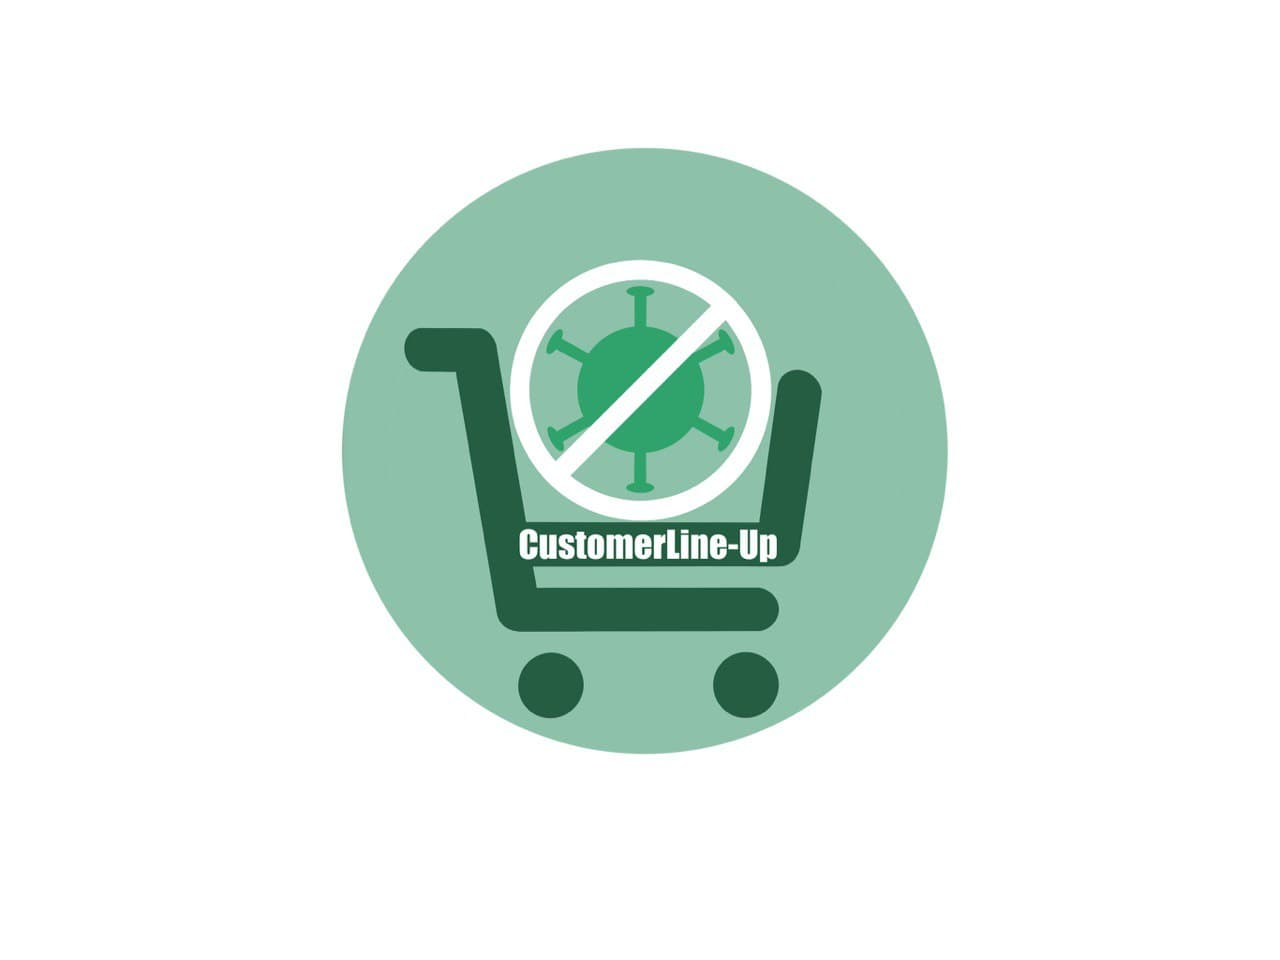
\includegraphics[scale=0.25]{img/logo.jpg}
\end{figure}
\end{center}
\vspace*{\fill}
\end{titlepage}

\normalsize


\newpage
\tableofcontents
\newpage

\section{Introduction}
\subsection{Purpose}
After showing a general description of the CL-up application within the RASD, this document focuses on analyzing the system's architecture and design, in order to satisfy the various requirements stated in the previous document. The purpose of the document is to provide a functional description of the main architectural components, showing their runtime behaviour and interactions and their interfaces. This document is mainly intended to be used by the developers and testers.

\subsection{Scope}
Customer Line-up (CL-up) is an application that aims to allow accesses to Stores in a safe way. The objective is to avoid as much as possible queue formation outside the Stores and limits the number of people inside it in an efficient way. To pursue this goal, the application allows Users to register either as a Managers or Customers, providing services to both of them. Managers can create their Stores within the app and allow other Managers to help them in the organization of the Store rules. Tools are provided to allow Customers to book Visits or Tickets to the Stores remotely, allowing a greater and more efficient way for maintaining social distancing. This is done by the use of a virtual queue managed by the System, in which Customers' Reservations are stored and managed. In order to organize the various entrances in the Stores, an identifier for each Consumer will be used, that is a QRCode.\\ %The application provides also a fall-back option (Paper Tickets) and suggestions for Customers.
\\
More information can be found in the Chapter 1 of the RASD.

\newpage
\section{Architectural Design}
\subsection{Overview: High-level components and their interaction}
In this chapter the architectural structure of the System will be described. In Figure \ref{high_level_overview_img} the high level overview of the System is shown. In the next sections we will describe in detail the various components and their interactions.

\begin{figure}[h!]
\centering
	\centering
  	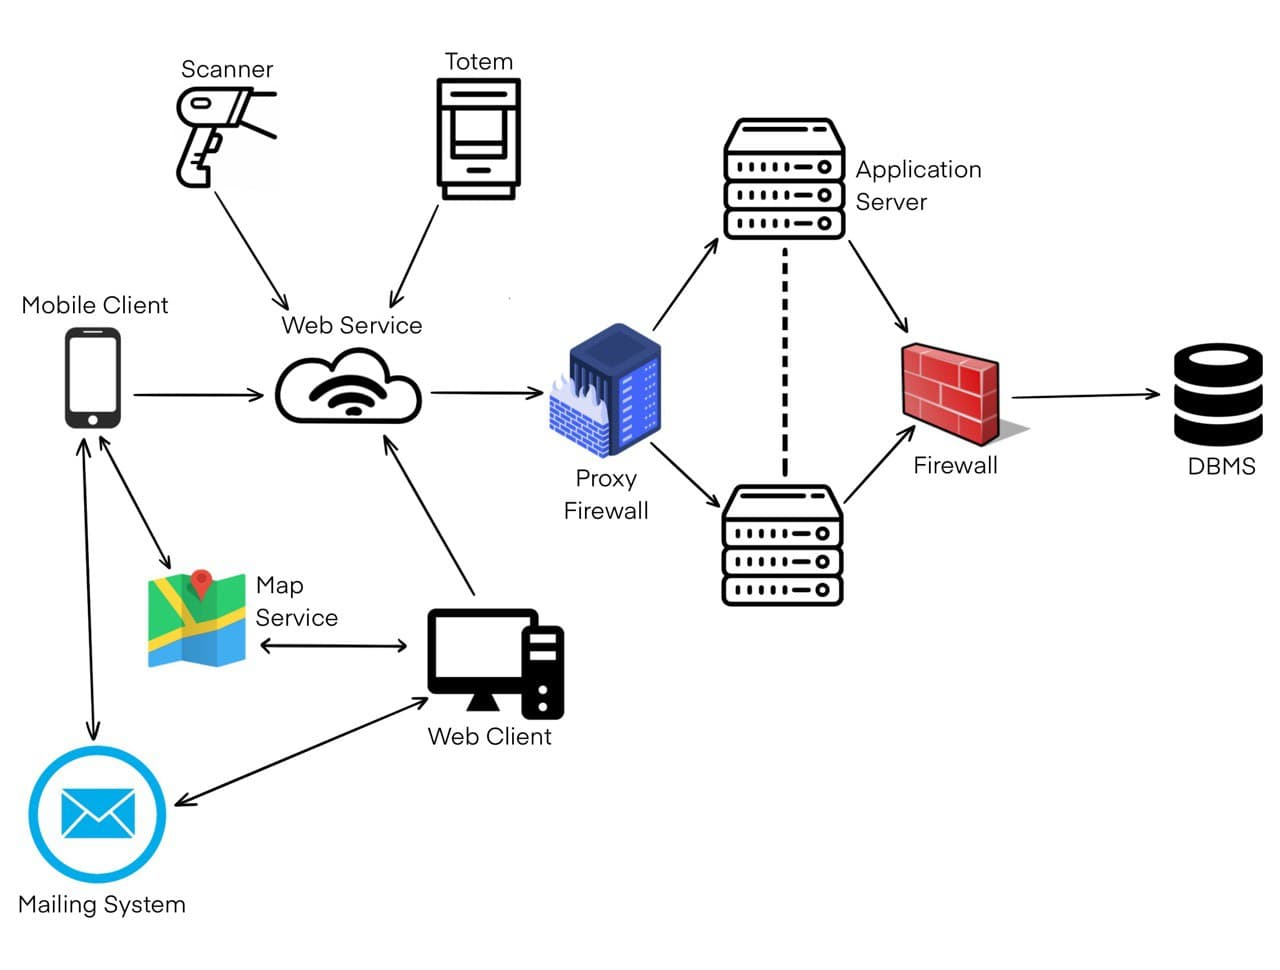
\includegraphics[height=0.4\textheight, scale=0.3, keepaspectratio]{img/high_level_overview.jpg}
	\caption{High-level overview of the System.}
 	\label{high_level_overview_img}
\end{figure}

\subsection{Component View}
To describe the internal modular structure of the components, we show how they are connected together in the UML component diagram in Figure \ref{comp_view_img} Components are wired together using an \textit{assembly connector} to connect the required interfave of one component with the provided interface of another component.

\begin{figure}[hbt]
\centering
	\centering
  	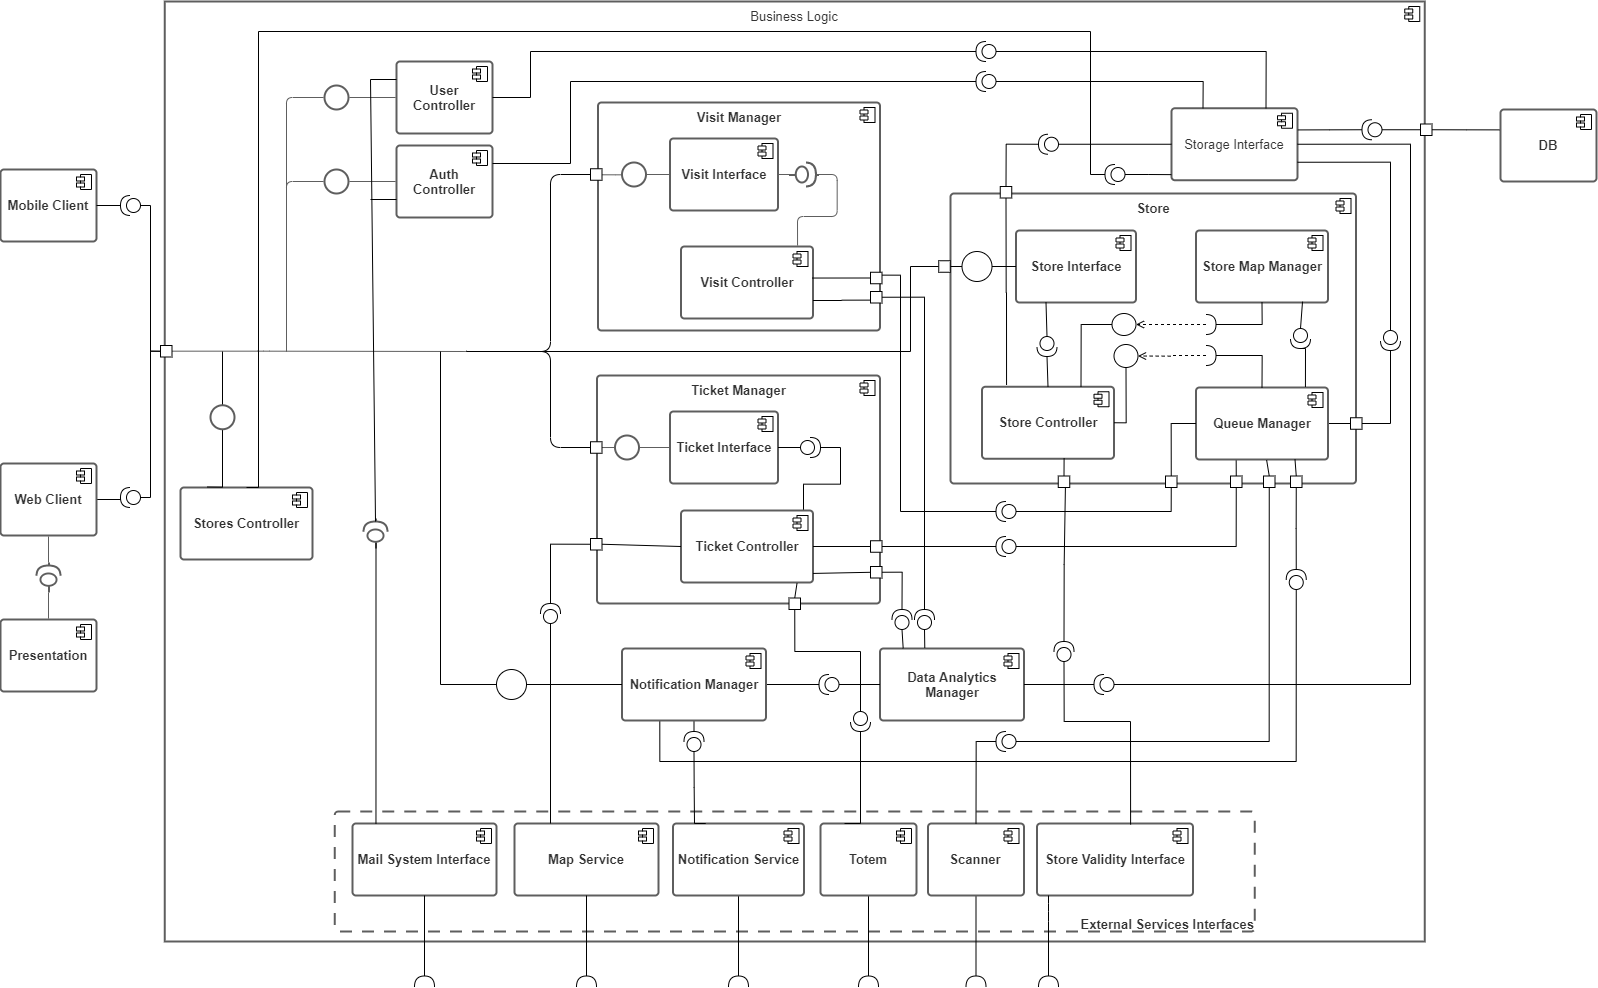
\includegraphics[height=0.4\textheight, scale=0.2, keepaspectratio]{img/component_view.png}
	\caption{Component diagram of the system.}
 	\label{comp_view_img}
\end{figure}

\begin{itemize}
    \item \label{cv:client}\textbf{Mobile Client} and \textbf{Web Client}: represents the two machines that accesses the entire System and it's functionalities. They both do not have important functions on their own, because we chose to implement them using a Thin Client approach.
    \item \textbf{Presentation}: it is used in order to display web pages of the application to a Web Client accessing through the browser. This layer only provides the structure of the user interface without accessing any data or application logic \lorenzo{forse metterei solo non accede all'application logic, perche' ai dati in qualche modo deve accederci per farli visualizzare su schermo (anche se puo' non sapere come siano stati estrapolati)}.
    \item \textbf{User Controller}: This component handles all the operations that affects the user data. It exposes method to change account credentials and stores them in the database.
    \item \textbf{Auth Controller}: This component handles all the operation for the authentication such as registration process and login process. It communicate with DBMS through Storage Interface in order to retrieve and insert user credentials. During the registration process or change password this component use Mailing System Interface
    \item \textbf{Data Analytics Manager}: is a component used in order to analyze Customers habits. In practice is a Recommender System that takes care of showing to a Customer the Stores most appealing to him and the best duration value to be included in a Reservation.
    \item \textbf{Notification Manger}: is a component used in order to provide Notifications to the Customer, such as  Virtual Tickets departures, appealing time slots of specific Stores and suggestions.
    \item \textbf{Ticket Manager}: is a subsystem component in charge of managing Ticket requests:
    \begin{itemize}
        \item \textbf{Ticket Interface}: it exposes to the Customer an Interface for compiling the requested Ticket attributes.
        \item \textbf{Ticket Controller}: it checks the validity of the inserted Ticket's attributes requested. Moreover it communicates with the Queue Manager in order to verify the possibility to accomplish the request.
    \end{itemize}
    \item \textbf{Visit Manager}:is a subsystem component in charge of managing Visit requests:
    \begin{itemize}
        \item \textbf{Visit Interface}: it exposes to the Customer an Interface for compiling the requested Visit attributes.
        \item \textbf{Visit Controller}: it checks the validity of the inserted Visit's attributes requested. Moreover it communicates with the Queue Manager in order to verify the possibility to accomplish the request.
    \end{itemize}
    \item \textbf{DB}: it represents the DBMS, which provide an interface to read and store data. User credentials, Stores information and queues reservations are stored  in the database.
    \item \textbf{Storage Interface}: it provide methods to access to database. This interface is needed in order to decouple all the components from the DBMS technology.
    \item \textbf{Store}: is a subsystem component in charge of managing Store and its Queue:
    \begin{itemize}
        \item \textbf{Store Interface}: it exposes to the Manager an Interface for creating and managing Stores.
        \item \textbf{Store Controller}: it ensures that a Manager intending to become Owner of a Store within the application has the necessary authorizations, checking the validity of the information by acquiring specific credentials. \yasmin{dovrei collegarlo a un external service di verifica??}
        \item \textbf{Queue Manager}: this component receives requests for Reservations for the Store, checks that they can be placed in the queue and eventually inserts them. It communicates with the Ticket Controller, the Visit Controller, the Scanner and the Totem. It also communicate with the DB in order to retrieve and modify all the necessary information.
        \item \label{comp:storeMapMan} \textbf{Store Map Manager}: this component receives requests from the Customers who has already booked a Visit. It has to populate the map with the path that the Customer should follow during their Visit inside the Store. It communicates with the Queue Manager to look at the specified departments by other people during the time-slot of the Visit specified.
    \end{itemize}
    \item \textbf{External Services Interfaces}: this set of components have as main objective to make API calls to the necessary third party services:
    \begin{itemize}
        \item \textbf{Mailing System Interface}: is an interface in charge of sending confirmation mails at the end of the registration process to the User. It also can send other type of notification mails.
        \item \textbf{Map Service}: this service is used in order to retrieve the necessary information about a Customer position. This information is used by the Data Analytics System and by the Ticket Controller \yasmin{???? ripensaci bene}
        \item \textbf{Totem \yasmin{Interface ?? forse meglio}}: since the Totem of a Store has the task of issuing Paper Tickets, it needs to communicate with the Ticket Controller in order to make requests and allow the effective issue of the requested Ticket. This component is in charge of the communication.
        \item \textbf{Scanner}: the Scanner application has the task of reading QR codes of Customers and Paper Tickets so that it can control the entries and exits from the Store. In order for it to carry out the correct checks, it needs to communicate with the Queue Manager to obtain the right information. This component is in charge of the communication.
        \item \textbf{Store Validity Interface}: Is used in order to check that the created store is a real store. To do this, it has to verify Special Credentials provided from the Owner.
        
        \item \textbf{Notification Service}: Is used from Notification manager in order to send push notifications to client application.
    \end{itemize}
    
\end{itemize}

\subsection{Selected Architectural Styles and Patterns}
\textbf{Client-Server Architecture}\\
The Client-Server Architecture is a computing model in which multiple components work in strictly defined roles to communicate. This roles can be divided in two main categories: the Server that hosts, delivers and manages most of the resources and services, and the Client that exploits those services. This architecture is also known as a networking computing model because all the requests and services are delivered over a network. When the Client needs a service, sends a resource or process request to the Server over the network connection, which is then processed and delivered to the Client. A Client can be connected to several Servers, each providing a different set of services, and a Server can manage several Clients simultaneously.\\
\\
Although a network operating system is needed, the Client-Server Architecure is characterized by several advantages that make it a good choice. First of all, thanks to the presence of a network that integrates various components, the System can be defined as distributed. Therefore, it's easy to replace, repair, upgrade and relocate a Server while Client remains unaffected. We can therefore say that this architecture is characterized by good scalability and maintanability. The other advantage is the security: indeed Servers control accesses and resources to ensure that only authorized Clients can access or manipulate data.\\
\\
\textbf{Three-Tiered Architecture}\\
The Three-tiered Architecture is a specific type of Client-Server system. It is a type of software architecture which is composed of three “tiers” or “layers” of logical computing:
\begin{itemize}
\item \textit{Presentation Tier}: is the front end layer and consists of user interface which displays content and information useful to an end user. This is the top-most tier and the only one accessible from the Client.
\item \textit{Application Tier}: contains the functional business logic of the application, it controls the application’s core functionality.
\item \textit{Data Tier}: comprises of the database/data storage system. It includes the data persistence mechanisms and the data access layer. In practice it is the layer that exposes the data. 
\end{itemize}
\begin{figure}[h!]
\centering
	\centering
  	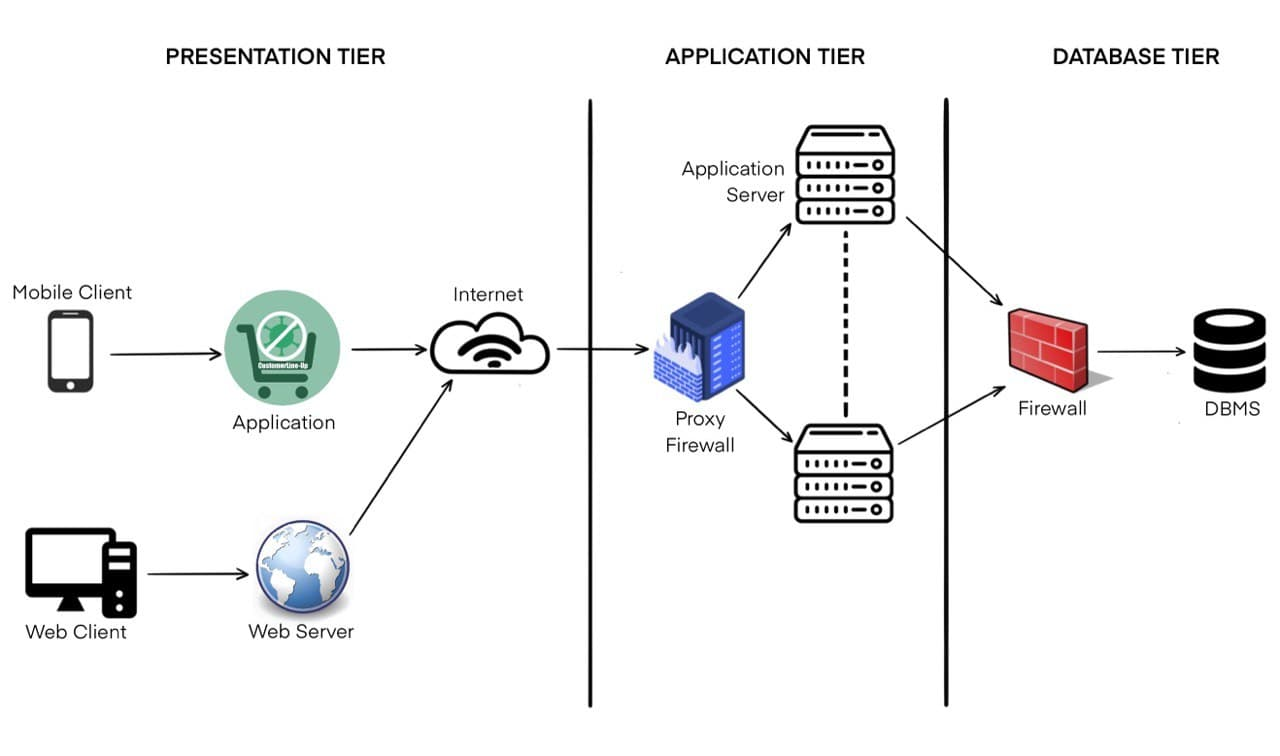
\includegraphics[height=0.35\textheight, scale=0.2, keepaspectratio]{img/three_tier_architecture.jpg} 
	\caption{Three Tier Architecture schema.}
 	\label{three_tier_architecture}
\end{figure}
The benefits of using a Three-Tier Architecture are many, including speed of development, scalability, performance and availability. Indees, modularizing different tiers of an application, gives the possibility to cìthe development team to develop the product with greater speed, because a specific layer can be upgraded with minimal impact on the other layers. In this way separate teams of the development team can focus on different components. Another other big advantage as we said is the scalability. By separating different layers, you can scale and load balance each independently, improving overall performance with minimal resources.\\
\\
\textbf{Thin Client}\\
A Thin client is a computer that serves to remote into a server, which handles all the computational load. Since Thin Clients hand off the heavy lifting to a Server, they don't need to have large memory or powerful computing capabilities to run the application.\\
\\
Being CLup an application for mobile phones, characterized by low computational power and small memories, thanks to the choice of adopting Thin Client, an internet connection is sufficient to use the application itself. and this is because all the computation is moved to the Server side, also allowing a simplification of the font end implementation.\\
\\
\textbf{Reverse Proxy Design Pattern}\\
a reverse proxy is a type of proxy server that retrieves resources on behalf of a client from one or more servers. Typically it sits behind a firewall and directs client requests to the appropriate Server. A reverse proxy provides an additional level of abstraction and control to ensure the smooth flow of network traffic between clients and servers. The avantages on using a Reverse Proxy are, first of all load balancing. Indeed a Reverse Proxy distributes Client's requests across a group of servers in a manner that maximizes speed and capacity utilization while ensuring no one server is overloaded, which can degrade performance. Moreover it ensure security and anonymity, in fact a Reverse Proxy protects identities and acts as an additional defense against security attacks.\\
\\
\textbf{REST: REpresentational State Transfer}\\
REST, or REpresentational State Transfer, is an architectural style for providing standards between computer systems on the web, making it easier for systems to communicate with each other. It is characterized by two main features: statelessness and the separation of concerns between Client and Server. In the REST architectural style, the implementation of the client and the implementation of the server can be done independently, that means that there can be done changes on one side without affecting the other side. As long as each side knows what format of messages to send to the other, they can be kept modular and separate. This improve the flexibility, the scalability and  additionally the separation allows each component the ability to evolve independently. Systems that follow the REST paradigm are stateless, meaning that the Server does not need to know anything about what state the Client is in and vice versa. In this way, both the server and the client can understand any message received, even without seeing previous messages. REST requires that a Client makes a HTTP request to the Server in order to retrieve or modify data on the server.\\
\\
\textbf{MVC Design Pattern}\\
Model–view–controller or MVC is a software design pattern commonly used for developing software systems. It specifies that the program logic of an application consist of three interconnected elements: model, view and controller. The \textit{model} directly manages data and rules of the application, it contains no logic describing how to present the data to a user. The \textit{view} presents the model's data to the user, it knows how to access the model’s data, but it does not know what this data means or what the user can do to manipulate it. And finally the \textit{controller} that stays between the view and the model, it listens to events and executes the appropriate reaction to these events.\\
\\
Usually this approach 
supports the choice of the Thin Client, that places almost the entire model, view and controller logic on the Server. MVC allows full encapsulation of objects. Furthemore, MVC provides decopuling of its components, which means that multiple developers can work simultaneously on the model, controller and views.\\
\\
\textbf{Relational DBMS}\\
A relational database is a digital database based on the relational model of data. This model organizes data into one or more tables of columns and rows, with a unique key identifying each row. A relational database organizes data into tables in a way for which you can retrieve an entirely new table from data in one or more tables with a single query. Another benefit of the relational database approach is that this type of databases support SQL, which is an easy human-readable language that enables CRUD operations for the storage.\giovanni{Questa frase non mi piace} \yasmin{questa che inizia a dx? come mai?}All of this make Relational databases a good choice for applications that involve several transactions at a time. Relational databases allow you to change the schema or how you model data on the fly, and it also eliminate data redundancy. The choice is also reinforced by the fact that data are structured.
\\
\paragraph{Firebase?}
\yasmin{devo aggiungere firebase? io non lo metterei.. forse lo metterei come CONSIGLIO in other design decisions} \lorenzo{Dovrebbe essere abbastanza uno standard dal punto di vista delle push notification.}
To send Push notification to the user for the suggestions to the Store to Visit and the updates on the reservations we use FCM - firebase cloud messaging.

\subsection{Other Design Decisions}
\subsubsection{The Queue Scaling Process}
One of the focal points of CLup is the creation of a good queuing mechanism for Consumers in order to enter the various Stores. But what exactly is meant by 'good'? First of all, good means that it takes into consideration that each Store will have its own personal queue, we generally want the queue and the entrances to be made in such a way as to allow simultaneous entry only to a number of Consumers equal to Capacity of each Store. It is also very important to keep in mind that one of the intentions of the application is to give a reasonable and as correct as possible departure time to all those Customers who have booked a Virtual Ticket remotely and must leave from the place in which they are in time to get to the Store for their turn. Other factors to take into consideration for a good construction of our queue are:
\begin{itemize}
\item All those who have a Paper Ticket will not be able to have an update on their time of entry to the Store.
\item Consumers who have booked a Visit must have priority of entry over those who have booked a Ticket.
\item Consumers who have booked a Paper Ticket have higher priority over those who have booked a Virtual Ticket.
\item People may take a different amount of time from the specified one to get out and the queue will have to react accordingly.
\item Some Consumer may not show up or may be late, and the queue will have to react accordingly.
\end{itemize}

Taking these factors into consideration, the following queuing mechanism was created. It is recommended that the following mechanism will be used when implementing the application by the development team.\\
\begin{figure}[hbt]
\centering
	\centering
  	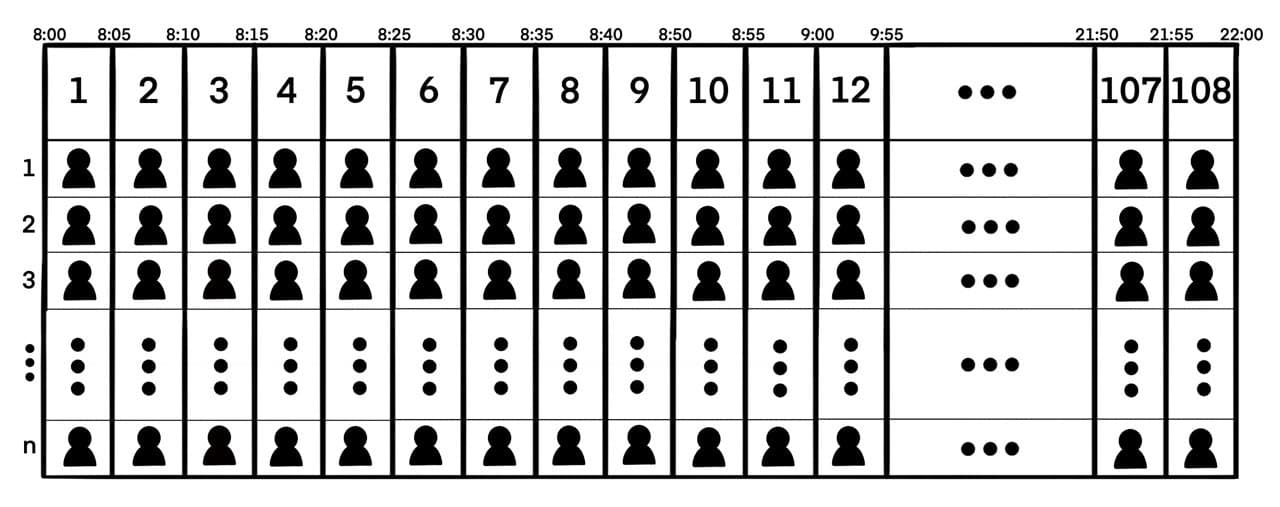
\includegraphics[height=0.2\textheight, scale=0.2, keepaspectratio]{img/queue/queue_general.jpg} 
	\caption{Example of a queue structure for one Store. The Store taken into consideration has as opening and closing hours 8:00-22:00. Consequently there are 108 Temporal Quantums of 5-minutes. Each quantum can hold up to \textit{n} people, with \textit{n} equal to the store capacity. In the example shown, all the quantum spaces have been occupied by a Consumer. No distinction was made between the various Consumers in this example.}
 	\label{entering}
\end{figure}
The queue is divided into Temporal Quantums. The beginning of the queue corresponds to the opening time of the Store, the end to its closing time. The time between the opening and closing hours is then divided into 5 minutes each. Each Temporal Quantum consists of a vector as long as the capacity of the Store. Whenever a certain Consumer requests a Ticket or a Visit, the temporal Quantums corresponding to its residence time are filled with a space, reducing the space available for other Consumers. In this way, entry will not be allowed to a number of people exceeding the Capacity available at any single time the Store is open. All the amounts of time of shopping for a single Consumer must be filled in so that they are sequential to each other (we obviously do not want a Consumer to enter and exit the Store several times to complete their shopping). Consequently, when a request for space is made, a search must be made in the queue to check where the first sequential set of spaces, large enough to satisfy the request of the Consumer, is located. Therefore, such a mechanism does not focus on the temporal precedence of the various requests but on the consistency of the satisfaction of the request itself. In fact, it may happen that a Consumer at time $t_1$ requests a space of 3 Temporal Quantum which will be booked in the queue temporally subsequent to the space of 2 Temporal Quantum booked by another Consumer at time $t_2$, and this is evidently because a space of 3 Temporal Quantums was not available before, but one of 2 yes.\\
\\
Until now, as long as Consumers come in and out at the appointed time, everything works fine. What does it mean to fill a series of Temporal Quantums? It means that at the start time of a certain Temporal Quantum the Store scanner expects to scan the QR Codes corresponding to the Consumers who have to enter in that Temporal Quantum. At the end time of the Temporal Quantum instead % (or to be precise a \yasmin{LITTLE BEFORE}, that is 30 seconds before to make him do the calculations ???)
the Scanner expects to scan the QR Codes of all the Consumers who at that moment should have concluded their shopping as indicated. However, it may happen that a Consumer takes longer than it should to complete their shopping, or less. Let's consider the following cases.\\
\\
In the case that a Consumer takes less than the pre-established time to exit the Store, basically no movement within the queue takes place. Their unused Temporal Quantums are simply freed up. In order for all Costumers with a Virtual Ticket to be provided with a good departure time, we do not want it to be possible for their filled Temporal Quantums to be anticipated. If so, it could happen that they are brought forward so much that they will no longer be able to leave on time from where they are to arrive on time for their turn. What happens is therefore simply a freeing of places within the unused Temporal Quantum, so that any other Consumers with new Tickets can occupy those spaces. In this way also the position of the Paper Tickets remains unchanged, and this is important as the entry time of the Paper Tickets cannot be updated because it is printed on a piece of Paper. In the event that a Consumer does not enter on time, that is in the event that his QR code is not scanned by the Scanner within the time included in his first Temporal Quantum filled, the consumer is considered late, and all his / her Temporal Quantums are released.\\
\\
In the case that a Consumer takes too long to exit the Store, that is when the System realizes that its Qr Code has not been scanned out within the pre-established time, it is necessary to scale the other Consumers in subsequent Temporal Quantums, so that he is given more time to finish the shopping and the limit of people inside the shop is not exceeded, that is the \textbf{Queue Scaling Process}. We will show the solution to the problem through the following example.\\
\\
Let's consider a Store with capacity 3 and opening hours 8:00, for which the following requests were made:
\begin{itemize}
    \item Consumer 2 has booked a 10 minute Visit between 8:05 and 8:15.
    \item Before the opening of the Store Consumer 1 requires a Virutal Ticket with a shopping time of 10 minutes (corresponding to two teporal quantums).
    \item Before the opening of the Store Consumer 3 requires a Virtual Ticket with a shopping time of 20 minutes.
    \item At 8:05 am Consumer 4 requests a Paper Ticket with a shopping time of 15 minutes.
    \item At 8:05 am Consumer 4 requests a Paper Ticket with a shopping time of 15 minutes.
    \item At 8:06 am Consumer 5 requests a Virtual Ticket with a shopping time of 15 minutes.
    \item At 8:07 am Consumer 6 requests a Virtual Ticket with a shopping time of 15 minutes.
    \item At 8:15 am Consumer 7 requests a Virtual Ticket with a shopping time of 10 minutes.
    \item At 8:16 am Consumer 8 requests a Virtual Ticket with a shopping time of 10 minutes.
    \item At 8:17 am Consumer 9 requests a Virtual Ticket with a shopping time of 10 minutes.
    \item At 8:20 am Consumer 10 requests a Virtual Ticket with a shopping time of 10 minutes.
    \item and so on..
\end{itemize}
\begin{figure}[hbt]
\centering
	\centering
  	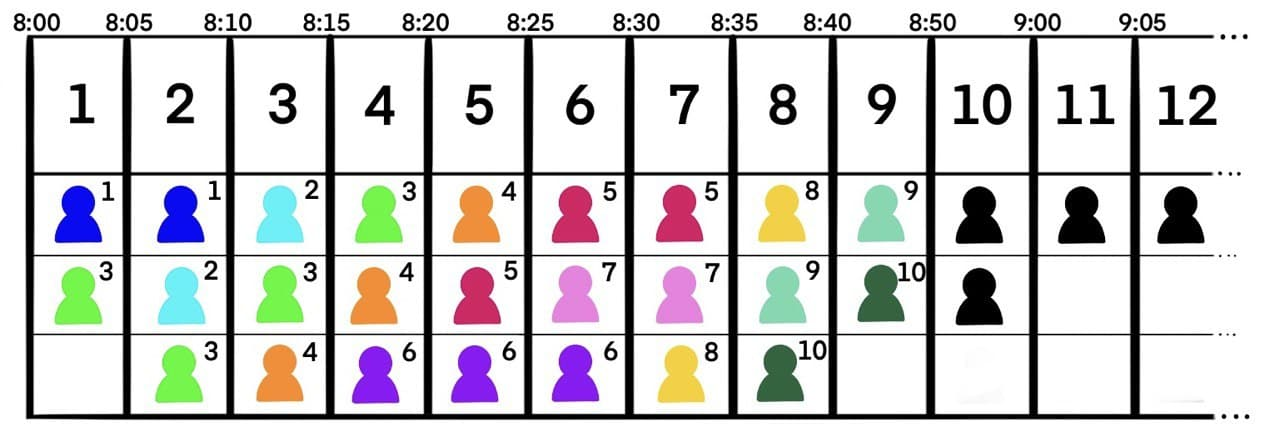
\includegraphics[height=0.15\textheight, scale=0.2, keepaspectratio]{img/queue/queue_ex1.jpg} 
	\caption{Queue Representation for the example described in this chapter. Each Consumer is characterized by its color and number in each space of the queue reserved for him.}
 	\label{queueex1}
\end{figure}
Let's consider the day time for which we arrive at the Temporal Quantum 4. At the end of this quantum Consumer 3 (which we will call $ C_3 $) should be out. Instead the Scanner did not receive any scan of the QR code of $ C_3 $. This means that $ C_3 $ hasn't come out yet. What happens then inside the queue?
\begin{figure}[hbt]
\centering
	\centering
  	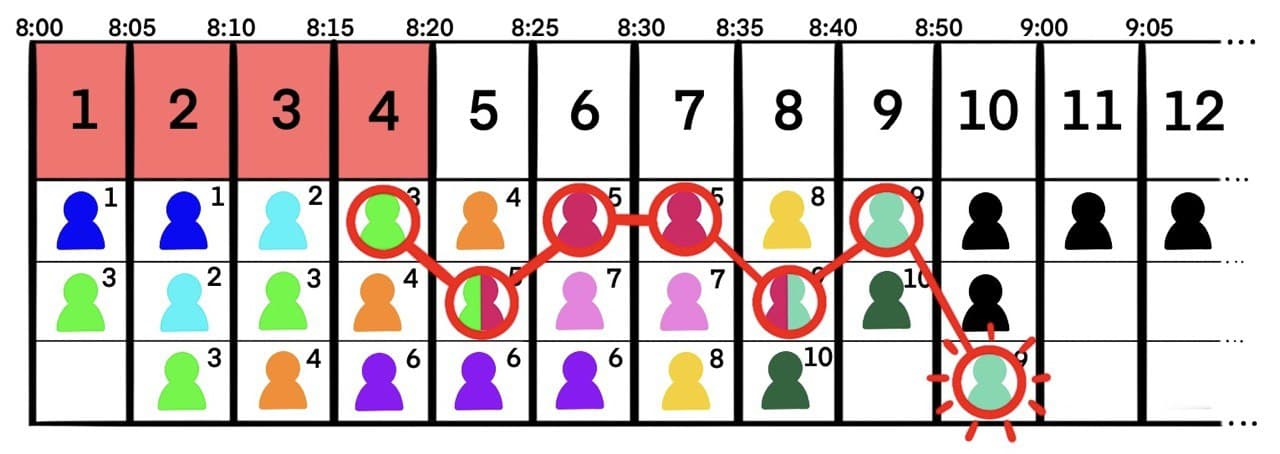
\includegraphics[height=0.15\textheight, scale=0.2, keepaspectratio]{img/queue/queue_ex2.jpg} 
	\caption{Representation of the queue for the example described in this chapter, specifically in the Temporal Quantum 4, highlighting the displacements caused by the Queue Scaling Process. A two-color character represents a Consumer passage that occupies that space. That is, the space that was previously occupied by the Consumer represented by the color on the right will now be occupied by the Consumer represented by the color on the left.}
 	\label{queueex2}
\end{figure}
$ C_3 $ didn't come out, so it needs more space. The queue will then give him a new Temporal Quantum. To do this it is necessary to check if there is an empty space at Temporal Quantum 5. If so, $ C_3 $ will take up that space. If this is not the case, it is necessary to choose a Consumer to be scaled. The rules for choosing the Consumer to scale, taking into consideration the previous considerations, are:
\begin{itemize}
    \item Consumers are analyzed starting from the last reserved.
    \item A Consumer who has already entered cannot be chosen.
    \item We are looking for a Consumer with a Virtual Ticket to be scaled.
    \item If not, we are looking for a Consumer with a Paper Ticket to be scaled up.
    \item In general, a Cunsumer with a Visit must not be scaled. If there is no Consumer with a Virtual Ticket or Paper Ticket to be scaled, a Visit will be scaled (this hypothesis is very remote).
\end{itemize}
    Taking these rules into consideration, let's look for a Consumer at the quantum 5 to scale to make space for $ C_3 $. $ C_6 $ has already entered the Store at quantum 4, so it cannot be scaled. $ C_5 $ hasn't entered yet and has reserved a Virtual Ticket, so it's perfect. $ C_5 $ will 'chase' its reserved spaces in the following Temporal Quantums until it reaches the last one, at Temporal Quantum 7, in which we will have to find a Consumer to scale down to the quantum 8 in order to let $ C_5 $ earn its place again. $ C_10 $ has not entered yet but has requested a Paper Ticket so we discard him for now. $ C_9 $ hasn't entered yet and has requested a Virtual Ticket, so it's perfect. At this point, $ C_9 $ behaves like $ C_5 $ for subsequent quantums. $ C_9 $ finally find an empty space at quantum 10, ending the scaling. If at quantum 5 $ C_3 $ had not yet left the Store, the scaling would repeat itself following the same rules, making $ C_7 $ scale, then $ C_10 $ and so on, until we find an empty space as before.
\begin{figure}[hbt]
\centering
	\centering
  	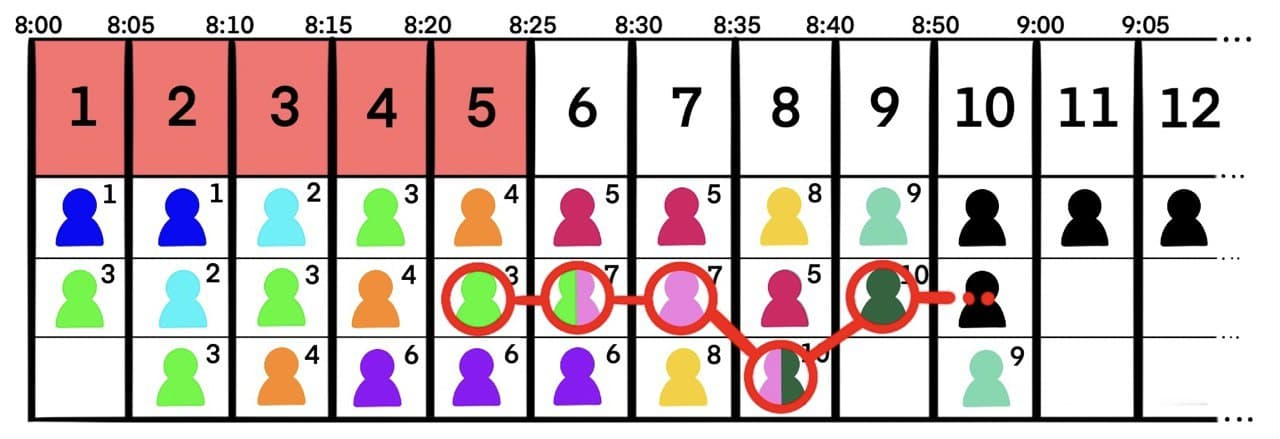
\includegraphics[height=0.15\textheight, scale=0.2, keepaspectratio]{img/queue/queue_ex3.jpg} 
	\caption{Representation of the queue for the example described in this chapter, specifically in the Temporal Quantum 5, highlighting the displacements caused by the Queue Scaling Process going on.}
 	\label{queueex3}
\end{figure}

What happens if during the scaling we reach the end of the queue, i.e. there is no longer enough space to satisfy the Consumer request? In this case the Consumer request will be eliminated as it is no longer possible to satisfy it. The Consumer will then be notified of this (through the CLup application if he is a Customer, or through the Scanner if he has a Paper Ticket). In order to eliminate as few Reservations as possible, a final space of non-bookable spaces is left in the queue, corresponding to the last 30 minutes of opening hours of the Store. In this way the first scales will certainly have space.\\
\\
The reason why a Visit is unlikely to be scaled is that the Manager can specify a percentage of Capacity of the Store that will be dedicated exclusively to reserve Tickets in every Temporal Quantum.

\subsubsection{The Map Generation Process}
In this section we give an example of how the map generation for the Visits could be generated.\newline
This map has two main objective: it wants to select a quick route for the Customer for him to go through all the departments that they have selected and it wants to minimize the possibility of overcrowding in the various departments. \newline
The creation of this map is delegated to the component Store Map Manager. \newline
This component is notified from the Queue Manager whenever a Visit is uploaded, deleted or modified (there has been a scaling event) \lorenzo{CONTROLLARE: scaling event o lo chiamiamo in un altro modo?} \yasmin{secondo me non serve specificare, basta 'modified' come hai scritto} \lorenzo{MMM, secondo me e' piu' chiaro se specifichiamo}. \yasmin{allora potremmo scrivere: there has been a scaling in the queue, senza dare un nome all'evento..?}\newline
In this explanation we will call the entrance and exit points of the Store as Departments. These type of departments are special because cannot be selected from the Customer.\newline 
Moreover, we will assume that the Customer spends the same amount of quantums in each \textit{normal} department, and only one quantum at the entrances and the exits (these two quantums are also considered to shared with the other departments). We assume that the Customer will be quick to switch department, thus no quantums will be assigned to check the movements between departments. \newline
This component will hold multiple data structure, which we will define as follow:
\begin{enumerate}
    \item QD: Marix \textit{\#Quantums in the queue X \#Departments in the Store}. In it there are written the number of people in a specific Departments for each Quantum in the Store (It is updated day by day, and there are only the quantums of each single day). This matrix makes the algorithm much more efficient in terms of run-time, but it is less efficient from the point of view of memory.
    \item MAP: it is the map of the store, which is a graph with the departments (also with entrances and exits). The links between the various departments indicate the available paths between each department. Each arc has a weight equal to 1.
    \item VCQ: it is a map (data structure), which maps the VisitID (primary key of each Visit), to its information. (The Map Manager will consider only the Visits in the current day, will delete the Visits of past days and will keep stored the future Visits). In particular there are the departments selected and a boolean IsMapped, to say if for this Visit has already been created a map.
    \item SP: Matrix (obtained for example with the Floyd–Warshall algorithm) which contains the shortest distances between each pair of node of MAP.
\end{enumerate}
This is how the Map Manager behaves after being notified by the Queue Manager:
\begin{enumerate}
    \item Insert: if a Visit is inserted, it is saved in VCQ and IsMapped is set to false. If the Visit will be in the current day, the map is generated. The department in VCQ of this Visit will be updated: an entrance and an exit will be added and the all list of departments will be ordered to reflect the computed path. The boolean IsMapped will be set to true. QD is updated accordingly. (with +1s in the correct positions, which are given by the quantums used by the Customer and the departments where they will be)
    \item Update: if a Visit is updated (due to scaling), if IsMapped is false, then VCQ is simply updated and nothing else happens. If IsMapped is true, than QD is updated (with -1s), from the departments we delete the entrance and the exit and the map is re-computed using the new data (thus QD is updated again with +1).
    \item Delete: if a Visit is deleted: if IsMapped is false, then the Visit is just deleted from VCQ. Otherwise, the Visit is deleted and QD is updated with -1.
\end{enumerate}

\vspace{0.4em}
\textbf{Create Map} \newline
\vspace{0.4em}

Let's define P[i, f]d as the average of the people in a department d from quantum i to quantum f (to compute it we just need the matrix QD).\newline
Steps for the algorithm:
\begin{enumerate}
    \item We compute the quantum used in the Visit, using the information given by the time-slot. We will call the initial quantum IQ and the final one FQ.
    \item We add to the departments selected by the user an entrance point and an exit point. For the entrance: we check the value of QD at quantum IQ for all possible entrances and we select the entrance with minimum value. For the exit: we check the the value of QD at quantum FQ for all possible exits and we select the exit with minimum value.
    \item We create a graph with only the departments selected by the Customer and the added entrance and exit as nodes. The graph is complete and each arc has a weight equal to the shortest path from one node to another in MAP (we can use the pre-computed SP to speed up the process)
    \item We add an extra node which is connected to the entrance node and the exit node with arcs of weight very small (possibly 0) and we will call this node S. Now, the problem of finding the shortest path from route to entrance to exit can be reduced to a TSP problem.
    \item Since TSP is an NP-hard problem, we use algorithms for its approximation (for example using MST, and NN greedy algorithm).
    \item Having computed one or more sub-optimal path for solving the problem of the shortest path, we select one considering that we want to decrease the probability that a large amount of people will be in the same department in the same quantums.
    \item We can easily compute which quantums will be assigned to each department (depending on their order in the path), since we assign to each selected department the same amount of quantums.
    \item We compute for each path the MAXP = maximum P[i, f]d (where i is the entrance quantum in the department d and f is the exit quantum of the department d).
    \item Considering both MAXP and the length of each path we infer (during the implementation we will need to find a suitable formula) which is the best path, we remove the node S from it, and we save the result in VCQ, setting IsMapped to true and updating QD accordigly.
    \item From this path we can easily compute the real path on MAP using, for example, Dijkstra algorithm to between each pair of ordered nodes.
\end{enumerate}

\vspace{0.4em}
\textbf{Example of Map Creation} \newline
\vspace{0.4em}
There has just been inserted a Visit which have:
\begin{enumerate}[label=-]
    \item Departments: 6 and 8
    \item Day: Current day (e.g. 15/12/2020)
    \item TimeSlot: 8:00-8:40
\end{enumerate}
The Store selected is represented in Figure [\ref{storeGraph}], and it has 6 departments, plus the entrance department 0 and two exit departments 5 and 7. \newline
In Figure [\ref{warshall}] there SP, computed from the Store Map Manager. Moreover in Figure [\ref{qd}] has been represented part of QD of the Store Map Manager.

\begin{figure}[H]
\centering
	\centering
  	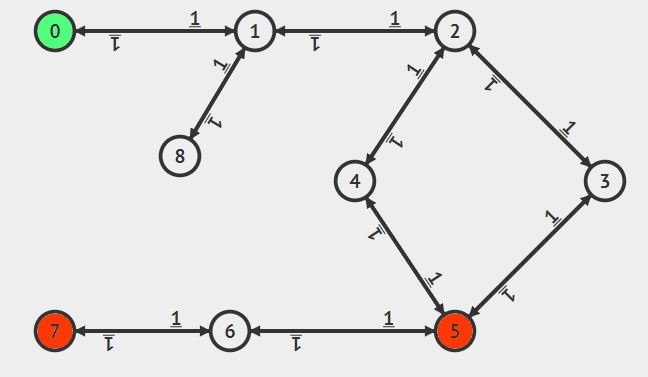
\includegraphics[height=0.4\textheight, scale=0.2, keepaspectratio]{img/alg_map_man/store_graph.JPG}
	\caption{MAP: Map of the Store}
 	\label{storeGraph}
\end{figure}
\begin{figure}[H]
\centering
	\centering
  	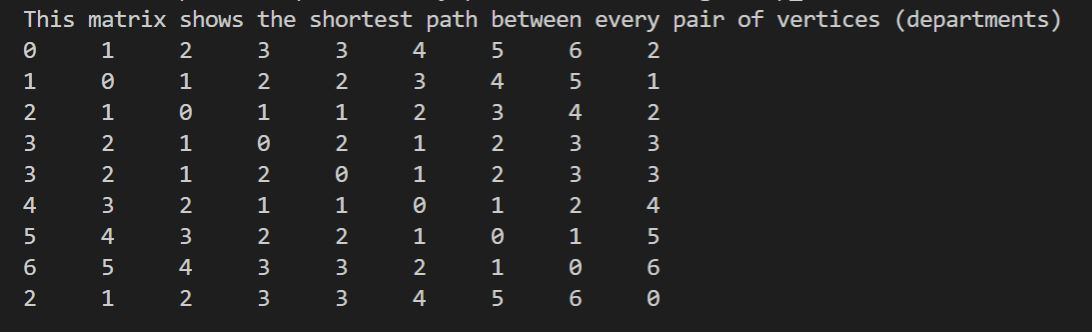
\includegraphics[height=0.2\textheight, scale=0.1, keepaspectratio]{img/alg_map_man/warshall_matr.JPG}
	\caption{SP: Shortest path between each pair of nodes in MAP}
 	\label{warshall}
\end{figure}
\begin{figure}[H]
\centering
	\centering
  	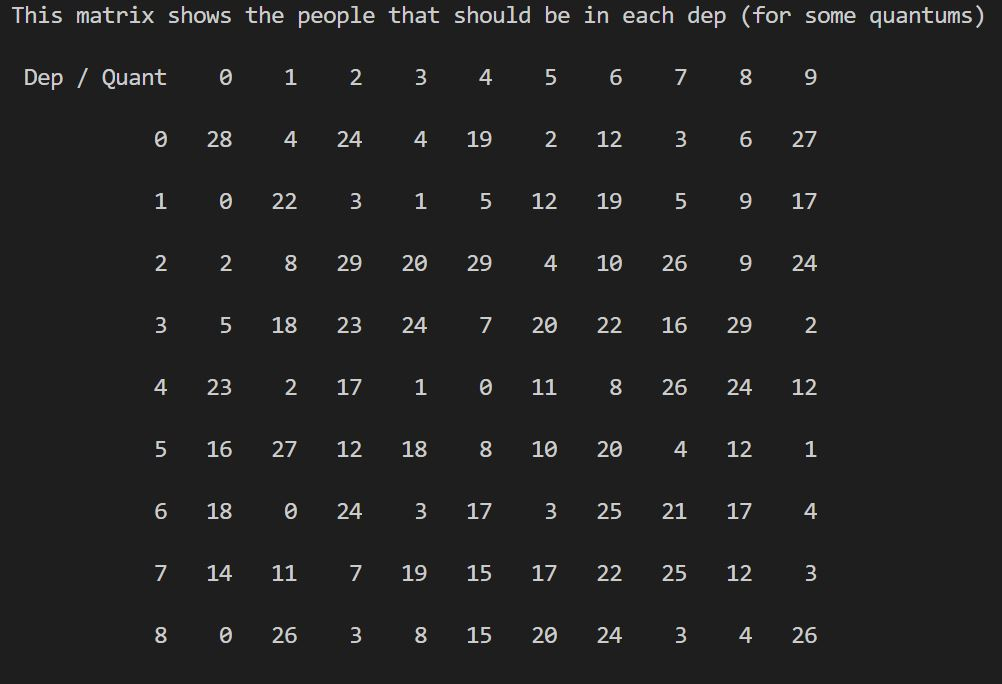
\includegraphics[height=0.4\textheight, scale=0.2, keepaspectratio]{img/alg_map_man/dep_quant_mat.JPG}
	\caption{QD: Estimated people in a specific department in a specific quantum}
 	\label{qd}
\end{figure}

Step for the algorithm:
\begin{enumerate}
    \item Each quantum has been defined to be 5 minutes-long, and that the time 8:00 is mapped to quantum 0.Thus this Visit lasts 8 quantums, from the $0^{th}$ to the $7th$. Since the Visit has only two departments, to each one of them will be assigned 8/2 = 4 quantums.
    \item We choose the entrance and exit dep. Since there is only one entrance department, 0 is selected. We have two exits. We select the exit which has the least amount of people at quantum 7 (from figure [\ref{qd}]), and it is 5 with 4 people.
    \item We create a graph with only the departments selected by the Customer and the added entrance and exit as nodes. The graph is complete and each arc has a weight equal to the shortest path from one node to another in MAP (we use the pre-computed SP (figure \ref{warshall}) to speed up the process). (figure [\ref{graphForTSP}])
    \item We add an extra node which is connected to the entrance node and the exit node with arcs of weight very small (possibly 0) and we will call this node S. Now, the problem of finding the shortest path from route to entrance to exit can be reduced to a TSP problem. (figure [\ref{graphForTSP}])
    \begin{figure}[H]
    \centering
    	\centering
      	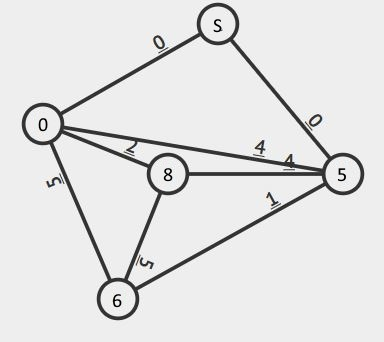
\includegraphics[height=0.4\textheight, scale=0.2, keepaspectratio]{img/alg_map_man/graph_for_tsp2.JPG}
    	\caption{Preparing graph for TSP}
     	\label{graphForTSP}
    \end{figure}
    \item In this example we just use the approximation of TSP using MST and we compute the MST using Prim's algorithm (Figure [\ref{mst}]).\newline
    If we read the nodes of the constructed MST in preorder-walk adding 0 at the end, we get: 0 - S - 5 - 6 - 8 - 0. It's length is = 0 + 2 + 5 + 1 + 0 = 8. We can see that if we traverse the path backwards and we delete the first two nodes, we obtain the path: 0 - 8 - 6 - 5. Which is what we were looking for. (and it still has length 8)
    \begin{figure}[H]
    \centering
    	\centering
      	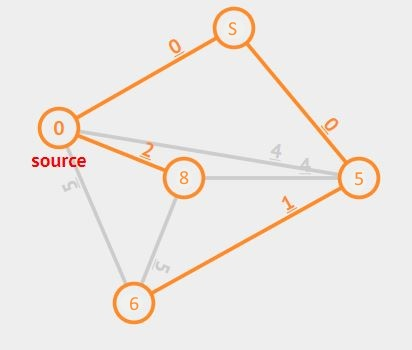
\includegraphics[height=0.4\textheight, scale=0.2, keepaspectratio]{img/alg_map_man/mst2.JPG}
    	\caption{MST of graph in figure \ref{graphForTSP}}
     	\label{mst}
    \end{figure}
    \item Since in this example we compute a single path, we would not need to check P[i, f]d in each department, but to better understand the algorithm, we now compute MAXP anyway. Since the first real department to be visited is 8, to it will be assigned the quantums from 0 to 3 included, and to department 5 will be assigned the quantums from 4 to 7 included \newline
    $MAXP = \max{\floor{(0 + 26 + 3 + 8)/4}, \floor{(8 + 10 + 20 + 4)/4}} = \max{9, 10} = 10$.
    \item Given the best path, we remove node S from it, and we save the result in VCQ, setting IsMapped to true and updating QD accordigly: (we add 1 to: (0, 0), (5, 7), (8, from 0 to 3 included), (6, from 4 to 7 included)).
    \item From this path we can easily compute the real path on MAP using, for example, Dijkstra algorithm to between each pair of ordered nodes. (figure \ref{afterDij})
    \begin{figure}[H]
    \centering
    	\centering
      	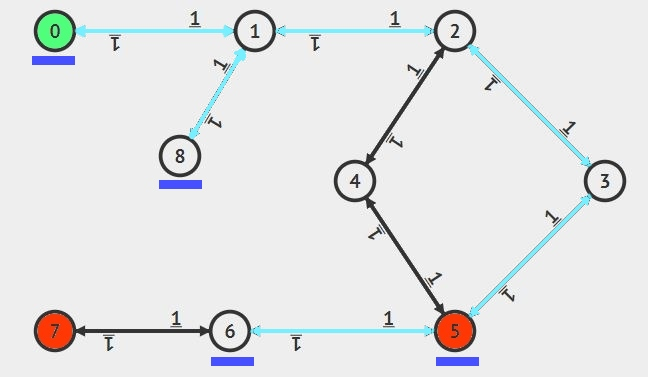
\includegraphics[height=0.4\textheight, scale=0.2, keepaspectratio]{img/alg_map_man/store_graph_PATH.JPG}
    	\caption{Created map for the Visit}
     	\label{afterDij}
    \end{figure}
\end{enumerate}

\vspace{0.4em}
\textbf{Final Considerations on the Map Creation} \newline
\vspace{0.4em}

The approach used does not give as an optimal solution neither for the shortest path problem nor for the overcrowding one. It tries to give a sub-optimal problems. Since the overcrowding that we mostly want to avoid is the one at the entrances and at the exits (so that a minor number of queues is generated), both entrance and exit are computed looking only at the estimated amount of people that should use them at a given quantum. \newline
To achieve the optimal solution for the shortest path problem, we should have used a brute-foce algorithm with time complexity O(n!), which would constraint the possible number of departments that the user can select to 9-10. Since the system could be used by large Stores, we thought, that we should give a more efficient solution. It is though possible to apply different algorithms, basing the choice on the number of selected departments in the Visit (thus, it is possible to solve TSP chosing a different algorithm from the one in the example).


\newpage
\section{User Interface Design}

\subsection{Mockup}
\begin{figure}[h!]
\centering
\begin{subfigure}
	\centering
  	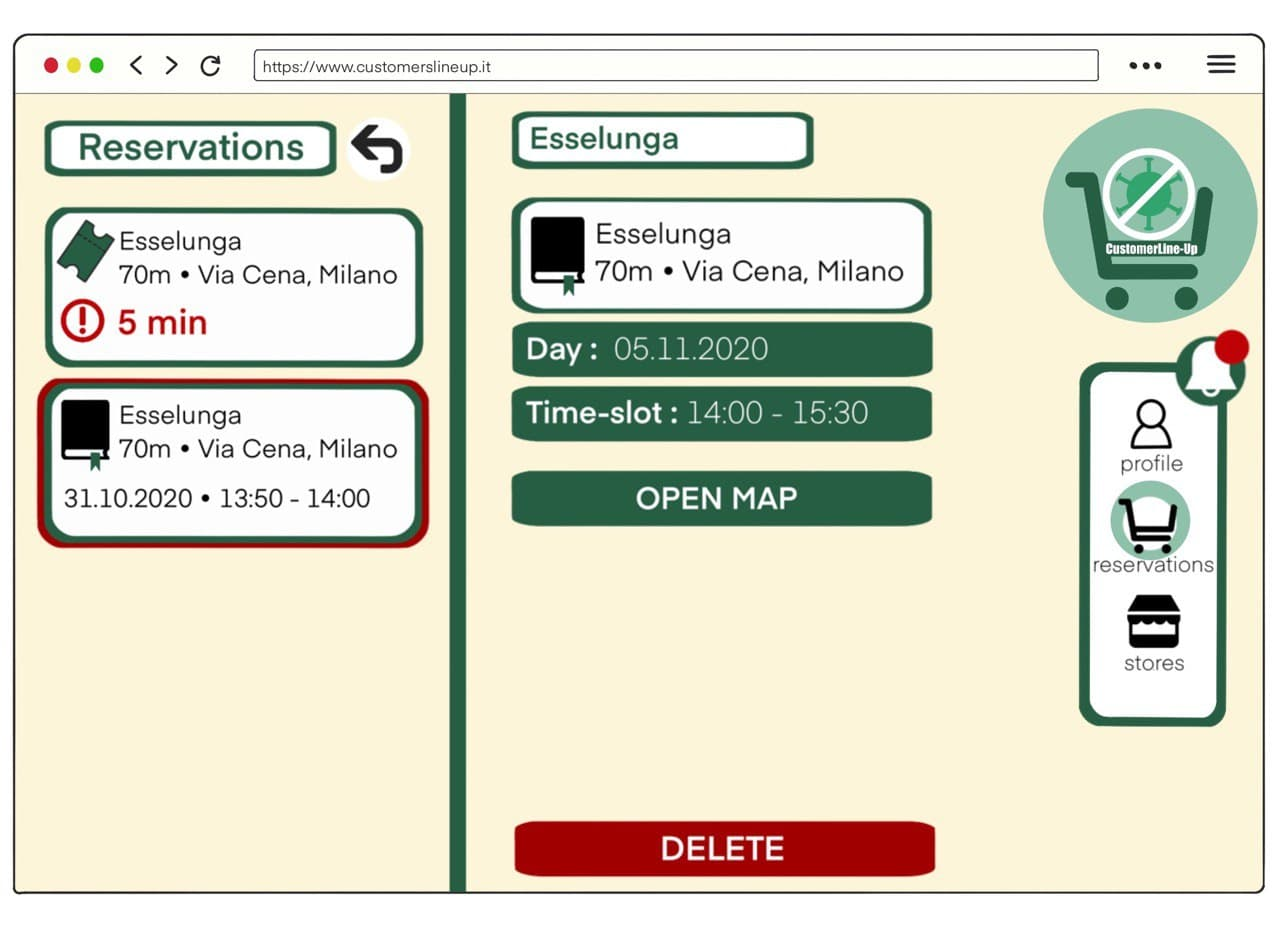
\includegraphics[height=0.4\textheight, scale=0.2, keepaspectratio]{img/customer_interface.jpg} 
 \end{subfigure}
 \begin{subfigure}
	\centering
  	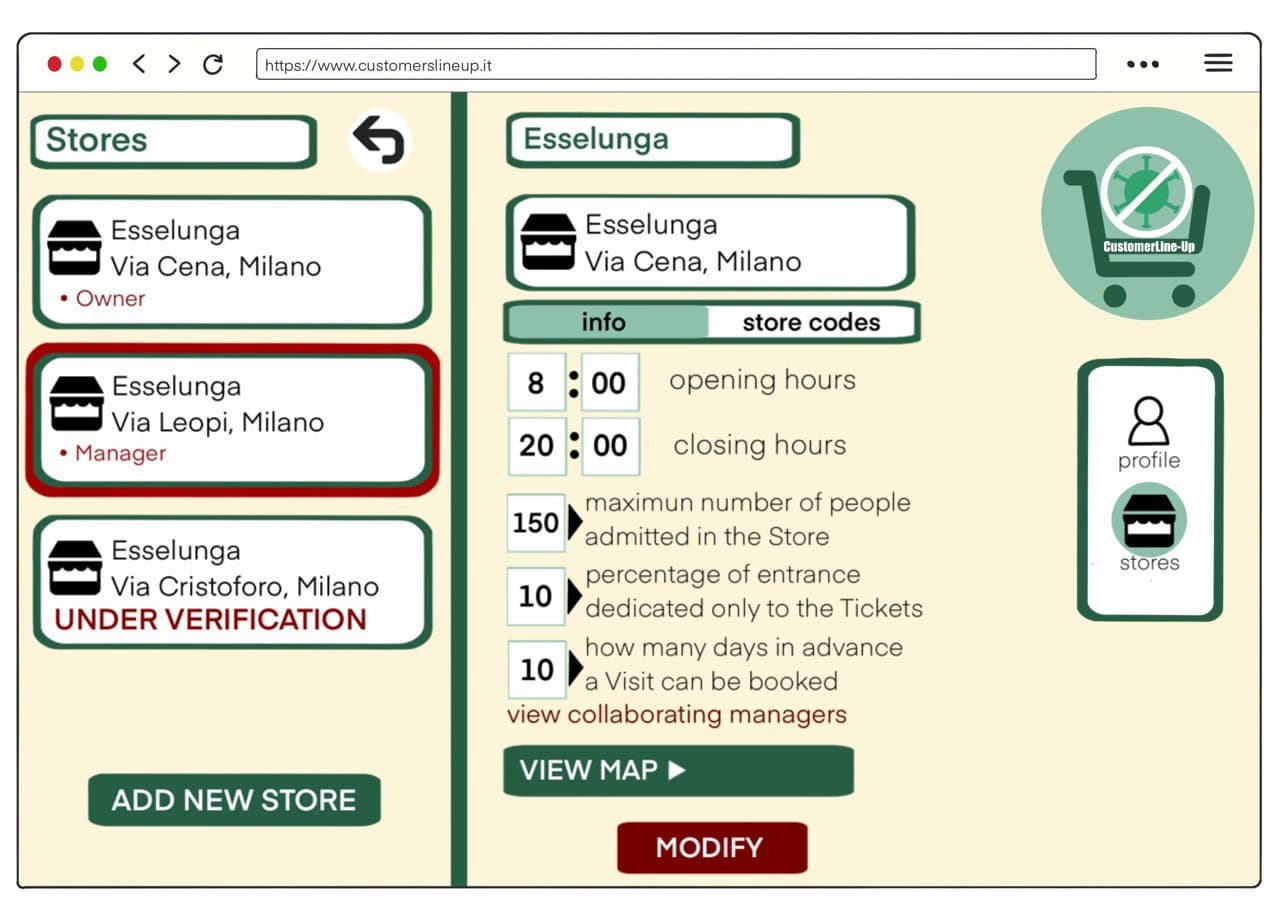
\includegraphics[height=0.4\textheight, scale=0.2, keepaspectratio]{img/manager_interface.jpg}
 \end{subfigure}
	\caption{Web page graphics.}
 	\label{web_graphics}
\end{figure}

\subsection{User Experience Diagram}
To better define the most important Users action within the application, we reported in Figure \ref{customer_experience} and in Figure \ref{manager_experience} two User Experience diagrams (UX), one for the Customer and one for the Manager. User Experience diagrams are diagrams that display the complete path a User takes when using a product, it refers to the functions and respective interfaces of the application.
\begin{figure}[h!]
\centering
	\centering
  	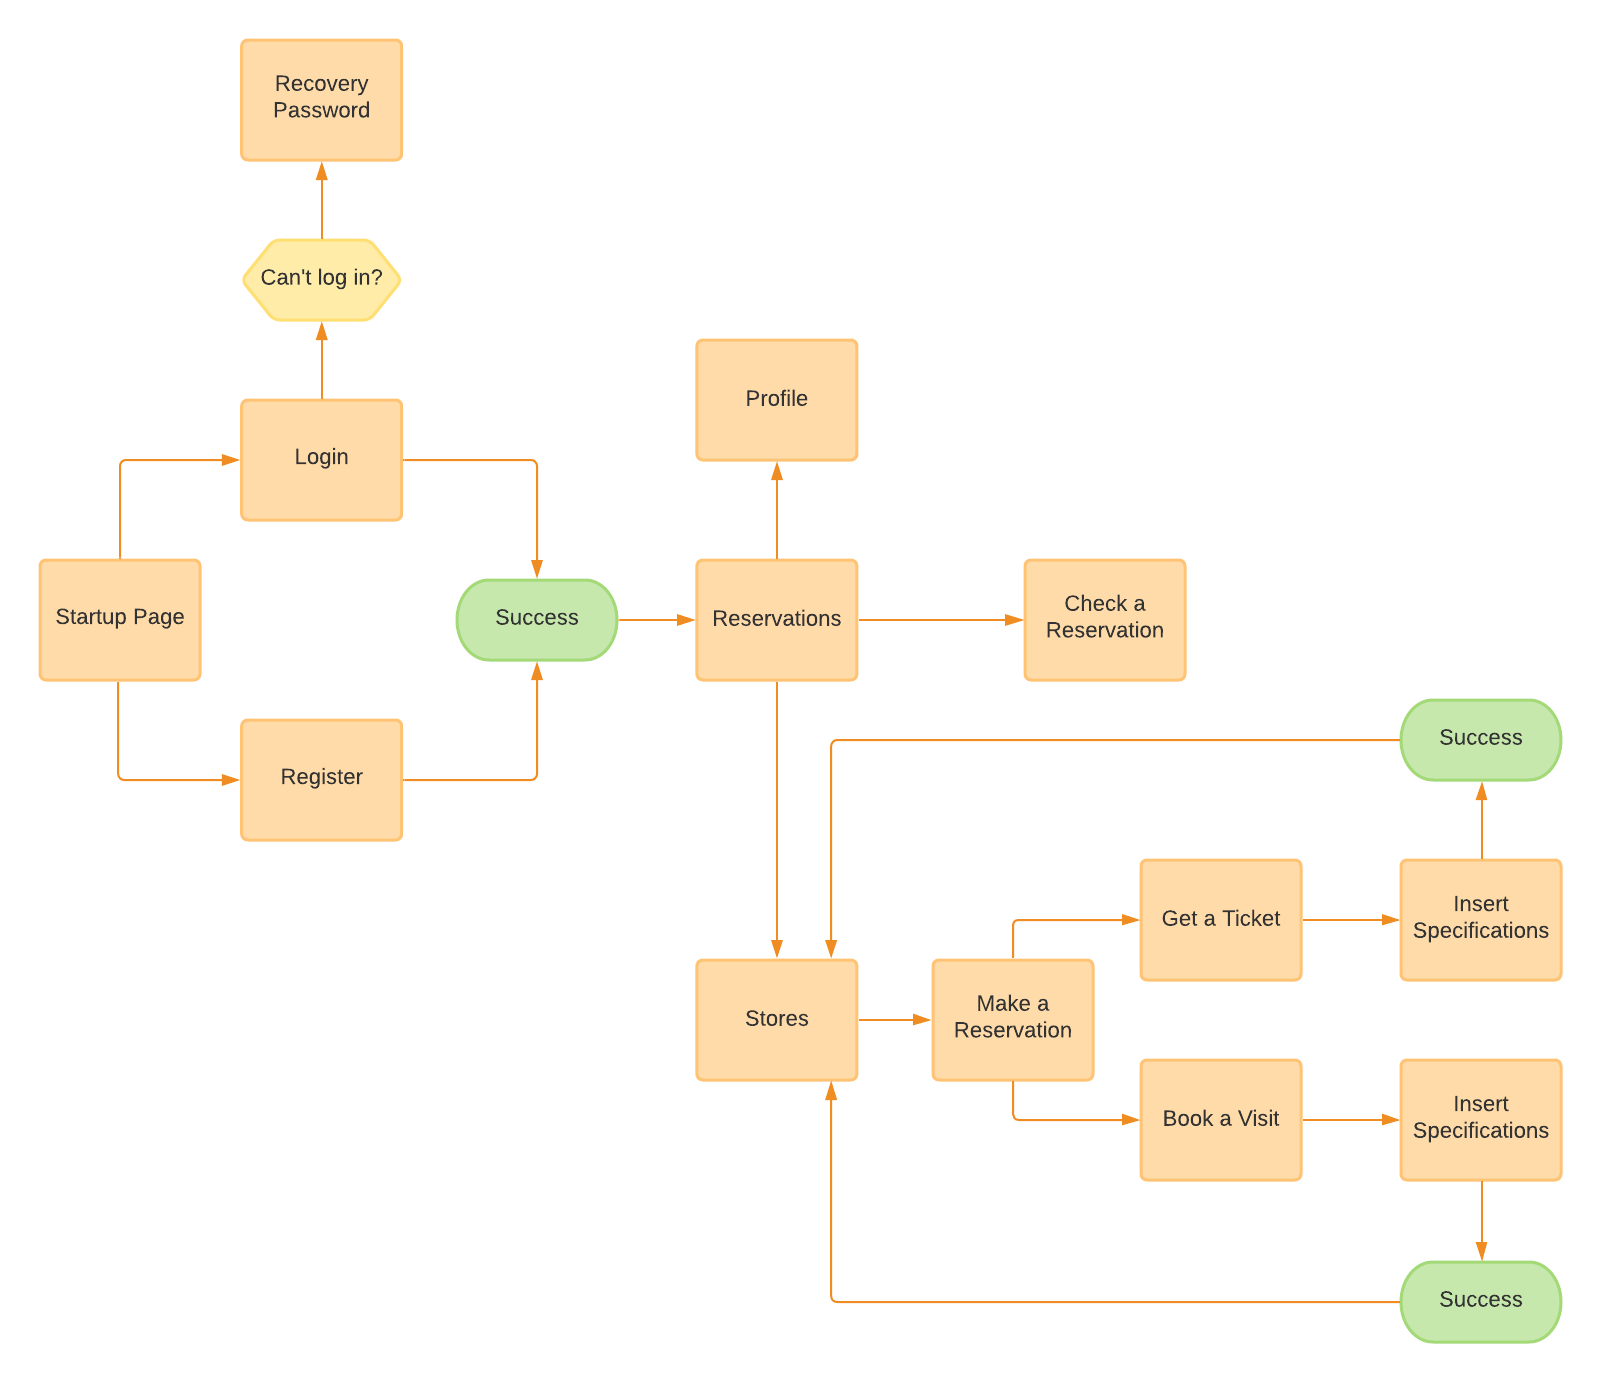
\includegraphics[height=0.5\textheight, scale=0.2, keepaspectratio]{img/customer_experience.png} 
  	\caption{UX flow of a Customer User.}
 	\label{customer_experience}
\end{figure}
\newpage
 \begin{figure}[h!]
	\centering
  	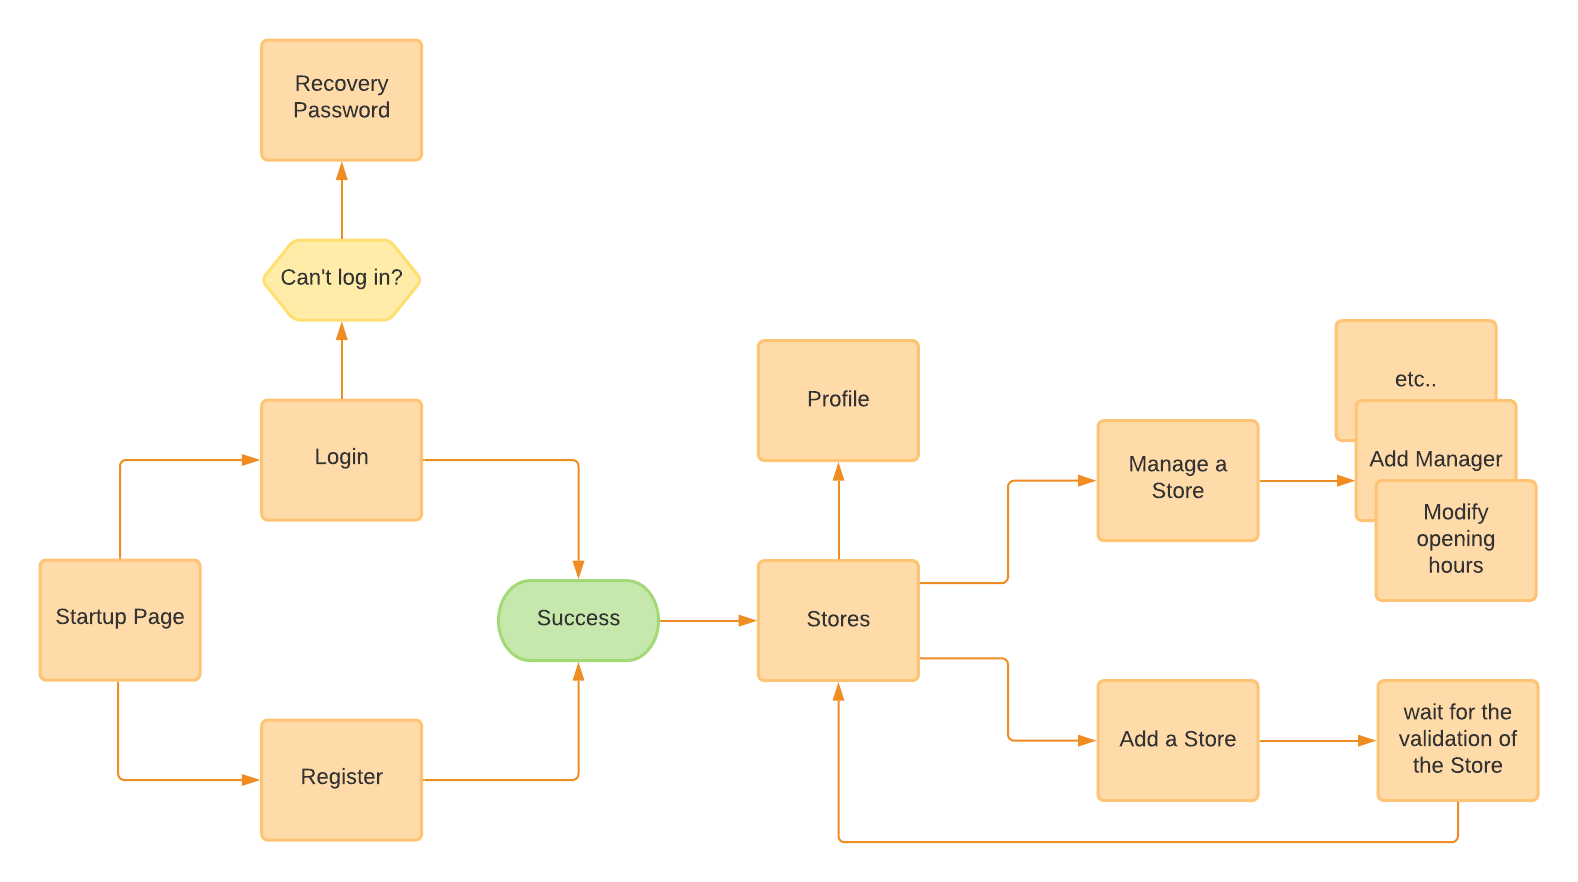
\includegraphics[height=0.35\textheight, scale=0.2, keepaspectratio]{img/manager_experience.png}
	\caption{UX flow of a Manager User.}
 	\label{manager_experience}
\end{figure}

\newpage
\section{Requirements Traceability}
Within the following document, the design and architectural choices have been made in order to satisfy the requirements and the various specifications contained in the RASD. In particular, in this chapter we will show the link that the System components (that can be found in the DD) have with the goals and requirements (that can be found in the RASD).
\subsection{Functional Requirements}
In the following table is shown which components are necessary to satisfy the requirements. \yasmin{HELP!!! REQUIREMENTS 7,11,16,20,21,30 DOVE LI METTOOOOOOO}
\newcolumntype{g}{>{\columncolor[HTML]{CDFFCD}}c}
\newcolumntype{o}{>{\columncolor[HTML]{FFCC99}}c}
\begin{tabularx}{\linewidth}{| g || l |}
	\hline
	%\rule{0pt}{15pt} & \cellcolor[HTML]{ADFFC0} \textit{Allow Guests to authenticate as Manager or Customer}\\
	\rule{0pt}{15pt}&\cellcolor[HTML]{FFCC99} \\
	\large{\textbf{Auth Controller}} & \cellcolor[HTML]{FFCC99} R.1, R.2, R.3, R.4\lorenzo{, R7: forse potremmo pensare di farlo come un trigger a livello di database, dato che alla fine e' un codice (lo metterei semplicemente in auth controller, come viene creato un id per l'utente viene creato il qr code per l'utente)}\\
    & \cellcolor[HTML]{FFCC99}\\
	\hline
	\rule{0pt}{15pt}&\cellcolor[HTML]{FFCC99} \\
	\large{\textbf{User Controller}} & \cellcolor[HTML]{FFCC99} R.1, R.5, R.6, R.8, R.17 \lorenzo{forse toglierei R.1} \yasmin{non serve per la registrazione user controller?}\\
    & \cellcolor[HTML]{FFCC99}\\
	\hline
	\rule{0pt}{15pt}&\cellcolor[HTML]{FFCC99} \\
	\large{\textbf{Data Analytics Manager}} & \cellcolor[HTML]{FFCC99} R.14, R.19, R.31\\
    & \cellcolor[HTML]{FFCC99}\\
	\hline
	 \rule{0pt}{15pt}&\cellcolor[HTML]{FFCC99} \\
	\large{\textbf{Notification Manager}} & \cellcolor[HTML]{FFCC99} R.19 \lorenzo{R.30: non ci sono i sottopunti, ma forse lo aggiungerei. perche' se ci sono degli update in visits o tickets dal punto di vista della coda, l'utente deve essere notificato.}\\
    & \cellcolor[HTML]{FFCC99}\\
	\hline
	\rule{0pt}{15pt}&\cellcolor[HTML]{FFCC99} \\
	\large{\textbf{Ticket Interface}} & \cellcolor[HTML]{FFCC99} R.9, R12 \lorenzo{R.30: stesso motivo di sopra}\\
    & \cellcolor[HTML]{FFCC99}\\
	\hline
	\rule{0pt}{15pt}&\cellcolor[HTML]{FFCC99} \\
	\large{\textbf{Ticker Controller}} & \cellcolor[HTML]{FFCC99} R.9, R.10\lorenzo{, R.11, R.14}\\
    & \cellcolor[HTML]{FFCC99}\\
	\hline
	\rule{0pt}{15pt}&\cellcolor[HTML]{FFCC99} \\
	\large{\textbf{Visit Interface}} & \cellcolor[HTML]{FFCC99} R.13\\
    & \cellcolor[HTML]{FFCC99}\\
	\hline
	\rule{0pt}{15pt}&\cellcolor[HTML]{FFCC99} \\
	\large{\textbf{Visit Controller}} & \cellcolor[HTML]{FFCC99} R.13, R.15\lorenzo{, R.14, R.20}\\
    & \cellcolor[HTML]{FFCC99}\\
	\hline
	\rule{0pt}{15pt}&\cellcolor[HTML]{FFCC99} \\
	\large{\textbf{Storage Interface}} & \cellcolor[HTML]{FFCC99} R.1, R.4, R.5, R.6, R.8, R.9, R.10, \\
	& \cellcolor[HTML]{FFCC99} R.13, R.22, R.23, R.24, R.26, R.27, R.28 \lorenzo{, R.21}\\
    & \cellcolor[HTML]{FFCC99}\\
	\hline
	\rule{0pt}{15pt}&\cellcolor[HTML]{FFCC99} \\
	\large{\textbf{Store Interface}} & \cellcolor[HTML]{FFCC99} R.22, R.23, R.24, R.26, R.27\\
    & \cellcolor[HTML]{FFCC99}\\
	\hline
	\rule{0pt}{15pt}&\cellcolor[HTML]{FFCC99} \\
	\large{\textbf{Store Controller}} & \cellcolor[HTML]{FFCC99} R.22, R.24, R.26, R.27\\
    & \cellcolor[HTML]{FFCC99}\\
	\hline
	\rule{0pt}{15pt}&\cellcolor[HTML]{FFCC99} \\
	\large{\textbf{Queue Manager}} & \cellcolor[HTML]{FFCC99} R.9, R.10, R.13, R.15, R.28, R.29\lorenzo{, R.21}\\
    & \cellcolor[HTML]{FFCC99}\\
	\hline
	\rule{0pt}{15pt}&\cellcolor[HTML]{FFCC99} \\
	\large{\textbf{Store Map Manager}} & \cellcolor[HTML]{FFCC99} R.13, R.15\\
    & \cellcolor[HTML]{FFCC99}\\
	\hline
	\rule{0pt}{15pt}&\cellcolor[HTML]{FFCC99} \\
	\large{\textbf{Mailing System Interface}} & \cellcolor[HTML]{FFCC99} R.3, R.6\\
    & \cellcolor[HTML]{FFCC99}\\
	\hline
	\rule{0pt}{15pt}&\cellcolor[HTML]{FFCC99} \\
	\large{\textbf{Map Service}} & \cellcolor[HTML]{FFCC99} R.9, R.10, R.18\\
    & \cellcolor[HTML]{FFCC99}\\
	\hline
	\rule{0pt}{15pt}&\cellcolor[HTML]{FFCC99} \\
	\large{\textbf{Totem \yasmin{Interface?}}} & \cellcolor[HTML]{FFCC99} R.29\\
    & \cellcolor[HTML]{FFCC99}\\
	\hline
	\rule{0pt}{15pt}&\cellcolor[HTML]{FFCC99} \\
	\large{\textbf{Scanner}} & \cellcolor[HTML]{FFCC99} R.28\\
    & \cellcolor[HTML]{FFCC99}\\
	\hline
	\rule{0pt}{15pt}&\cellcolor[HTML]{FFCC99} \\
	\large{\textbf{Store Validity Interface}} & \cellcolor[HTML]{FFCC99} R.22, R.24\\
    & \cellcolor[HTML]{FFCC99}\\
	\hline
	\rule{0pt}{15pt}&\cellcolor[HTML]{FFCC99} \\
	\large{\textbf{\lorenzo{Stores Controller}}} & \cellcolor[HTML]{FFCC99} \lorenzo{R.16} \yasmin{ma se stores contr permette di scegliere lo store giusto a cui collegarsi..}\\
    & \cellcolor[HTML]{FFCC99}\\
	\hline
	
    \caption{System's components and requirements mapping on goals.}
\end{tabularx}
%\captionof{table}{System's components and requirements mapping on goals.}
\vspace{5mm}
In order for the table to be understood, we briefly report in the table below the reference Functional Requirements whose more precise and exhaustive description can be found in the RASD.

\begin{tabularx}{\linewidth}{| o || l |}
    \hline
    R.1 & The User must be able to register or to log in if already registered.\\
    \hline
	R.2 & Check if the User credentials are valid.\\
	\hline
	R.3 & If the credentials are valid, the System sends a confirmation email, to let the\\
	& User activate their account.\\
	\hline
	R.4 & Allow to log in using personal credentials. \\
	\hline
	R.5 & Allow to change credentials, if the new credentials are in the right format. \\
	\hline
	R.6 & Allow to change password if it has been forgotten, through the personal email. \\
	\hline
	R.7 & Provide to each Customer a unique QR code which will be used as identifier\\
	& within the System.\\
	\hline
	R.8 & Users must have the possibility to delete their accounts. \\
	\hline
	R.9 & The Customer must be allowed to request a Ticket. \\
	\hline
	R.10 & For Customers who are requesting a Ticket, the System should \yasmin{act to provide it}. \\
	\hline
	R.11 & Each Customer can request only one Ticket. \\
	\hline
	R.12 & Every person on a Ticket can view the time in which they should enter the Store\\
	& and the indicated duration of their shopping. \\
	\hline
	R.13 & The Customer must be allowed to request a Visit.\\
	\hline
	R.14 & For long time Customers, while booking a Visit or a Ticket,\\
	& the System should infer, analyzing previous Reservations of that\\ 
	& Customer, the expected duration of the Visit or Ticket. \\
	\hline
	R.15 & The System should provide to the Customer a map of the Store.\\
	\hline
	R.16 & Allow Customers to consult their\\
	& pending requests.\\
	\hline
	R.17 & The Customer must be allowed to delete a Visit or a Ticket from his/her\\
	& pending requests.\\
	\hline
	R.18 & Use third party services to enable the localization of Customers and Stores. \\
	\hline
	R.19 & Notify Customers of available slots in a day-time range inferring information\\
	& from their previous Visits.\\
	\hline
	R.20 & Each Customer can book up to three Visits in a single day.\\
	\hline
	R.21 & If a Reservation is expired, or it has served its purpose, or it has been deleted,\\
	& it will be removed and will not be visible to the Customer anymore.\\
	\hline
	R.22 & Allow Managers to create Stores, becoming the Owner of the Store.\\
	\hline
	R.23 & Allow Owners to delete their Stores.\\
	\hline
	R.24 & Verify the Store creation, acquiring specific credentials (for instance a Certified\\
	& Email) that can be used to verify the validity of the Store and of the Manager.\\
	\hline
	R.25 & Allow the Owner and Managers to edit the Store.\\
	\hline
	R.26 & All the information about the Store can be updated by their Managers at anytime.\\
	\hline
	R.27 & Allow Managers to upload a map of their Stores.\\
	\hline
	R.28 & Provide a specific \textbf{Scanner App} to scan the QR codes of the Consumers and to\\
	& interact with the Queuing Mechanism.\\
	\hline
	R.29 & Provide a specific \textbf{Paper Tickets App} to generate paper tickets in the Store and\\
	& to interact with the Queuing Mechanism.\\
	\hline
	R.30 & Each Store has one and only one queue.\\
	\hline
	R.31 & Suggestions are based on the habits of the Customers, inferred by the Data\\
	& Analytics Manager.\\
	\hline
    
\end{tabularx}

\subsection{Non-Functional Requirements}
The Non-Functional Requirements of the application are defined in the Sections 3.3 and 3.5 of the RASD. Design choices like the Three-Tier Architecture acts to improve and respect the performances needed and in general to improve the software quality attributes.

\end{document}
